%% -*- coding:utf-8 -*-

\chapter{词汇功能语法}
%\chapter{Lexical Functional Grammar}
\label{Kapitel-LFG}

词汇功能语法(Lexical Functional Grammar,简称LFG)是上个世纪八十年代由Joan Bresnan和Ron Kaplan提出来的\citep{BK82a}。LFG是所谓的西海岸语言学的一个有机组成部分:不同于乔姆斯基任教的麻省理工学院,Joan Bresnan和Ron Kaplan在美国的西海岸工作(Joan Bresnan任教于斯坦福大学,而Ron Kaplan先后供职于帕罗奥图的施乐和加利福尼亚湾区Nuance的语言技术部门)。

\citet{BK82a}视LFG为一种心理语言学角度来看合理的、可以替换转换机制的分析方法。
请参考\ref{Abschnitt-Diskussion-Performanz}以了解更多基于心理语言学讨论的语言学理论的合理性的讨论。 

想了解更多的基于LFG来分析德语的工作,可参阅\citew{Berman96a-u,Berman2003a}和\citew{Cook2001a}。

LFG有着设计良好的形式理论基础\citep{KB82a-u,Kaplan95a},正是基于这一点,LFG工程实践也开展得较早并取得了不少成果
\citep*{FR83b,FR83a,Yasukawa1984a-u,BH86a-u,%
ED86a-u,% CHARON Parser
WA86a-u,%
Delmonte90a-u,% Italien
HHP91a-u,% Chinesisches kommerzielles System
Kohl92a-u,KGPRM92a-u,% ACORD project CHARON Generator
KM96a-u,%
Mayo97a-u,Mayo99a-u,%Konstanzer system
BS2005b-u,BSagot2005a-u,%SxLFG
Clement2009a-u,CK2001a-u% XLFG
}。

我们列举了一些已经实现出来的LFG语法片段:

\begin{itemize}
\item 阿拉伯语\il{Arabic} \citep{Attia2008a-u}、
\item 阿伦特语\il{Arrernte} \citep*{Dras2012a-u}、
\item 孟加拉语 \il{Bengali} \citep{SC97a-u}、
%\item Chinese\il{Mandarin Chinese}
\item 丹麦语\il{Danish} \citep{Oersnes2002b-u,OW2003a-u,OW2004a-u}、
\item 英语\il{English} \citep*{HHP91a-u,BDFK99a-u,RKKCMJ2002a-u,KM2007a-u}、
\item 法语\il{French} \citep*{Zweigenbaum91a-u,Frank96b-u,FZ2002a-u,BDFK99a-u,CK2001a-u,BSL2005a-u,SdA2016a-u,Alencar2017a-u}、
% Knueppel2001a-u
%
%
\item 格鲁吉亚语\il{Georgian} \citep{Meurer2009a-u}、
\item 德语 \citep{Rohrer96a,Berman96a-u,KR97a-u,BDFK99a-u,Dipper2003a-u,RF2006a,Forst2006a-u,Frank2006a-u,FR2009a-u}、
%\item Griechisch\il{Griechisch}、
\item 匈牙利语\il{Hungarian} \citep{LRT2010a-u}、
\item 印度尼西亚语\il{Indonesian} \citep*{AADMS2009a-u}、
\item 意大利语\il{Italian} \citep*{Delmonte90a-u,Mayo99a-u,Quaglia2012a-u}、
\item 爱尔兰语\il{Irish} \citep{Sulger2009a-u,Sulger2010a-u}、
\item 日语\il{Japanese} \citep*{HHP91a-u,MO2003a-u,Umemoto2006a-u}、
\item 韩语\il{Korean} \citep*{HHP91a-u}、
\item 马达加斯加语\il{Malagasy} \citep*{Randriamasimanana2006a-u,DLM2006a-u}、
\item 现代汉语\il{Mandarin Chinese} \citep*{HHP91a-u,FK2007a-u}、
\item Murrinh-Patha语\il{Murrinh-Patha} \citep{SN2012a-u}、
\item 挪威语\il{Norwegian} \citep*{DMR2005a}、
\item 波兰语\il{Polish} \citep*{PP2012a-u}、
\item 葡萄牙语\il{Portuguese} \citep{Alencar2004a-u,Alencar2013a-u,Alencar2015a-u}、
\item 西班牙语\il{Spanish} \citep{Mayo99a-u}、
\item 提格里尼亚语\il{Tigrinya} \citep{Kifle2012a-u}、
\item 土耳其语\il{Turkish} \citep{CO2006a-u}、
\item 匈牙利语\il{Hungarian} \citep*{LRT2010a-u,RLC2011a-u}、
\item 乌尔都语/北印度语\il{Urdu}\il{Hindi} \citep*{BHKR2007a-u,BBS2008a-u}、
\item 威尔士语\il{Welsh} \citep{MS2005a-u}
和
\item 沃洛夫语\il{Wolof} \citep{Dione2012b-u,Dione2013a-u}。
\end{itemize}
上述语法中很多都是基于ParGram开发的\footnote{
  \url{http://pargram.b.uib.no/research-groups/}。\zhdate{2015/10/01}。
} \citep*{BKNS99a-ed,BDKMR02a-u}。 
除了上述语法,一个针对北梭托语\il{Northern Sotho}的语法也正在研发\citep{Faasz2010a-u}。

很多LFG系统除了使用以语言学为准的语法,还使用统计模块
\isc{统计学}\is{statistics}。
这样的模块可以帮助搜索一个句子最为倾向的解读分析。统计模块可以增强语言处理的效率,也可以增强系统鲁棒性\citep{KRKMVC2004a-u,RKKCMJ2002a-u}。
Josef van Genabith在都柏林的团队目前正在研究如何从语料中自动约归出LFG语法\citep{JGCCR99a-u,DBCGW2005a-u,CBFDRCW2005a-u,CG2006a-u,GWG2007a-u,CBDRGW2008a-u,SvG2009a-u}。

\pagebreak
很多系统都提供在线测试功能,如:
\begin{itemize}
\item \url{http://iness.uib.no/xle-web/xle-web}

% Statistik Dublin
\item \url{http://lfg-demo.computing.dcu.ie/lfgparser.html}
\item \url{http://www.xlfg.org/}
\end{itemize}

\section{关于表示形式的一般说明}

\label{Abschnitt-Format-LFG}

LFG假设多层表征。\footnote{
  本节中英语例句及其分析选自于\citet{Dalrymple2001a-u}和\citet{Dalrymple2006a}。
}
其中最重要的是c-结构
\isc{c-结构}\is{c"=structure}和f-结构
\isc{f-结构}\is{f"=structure}。
c-结构是结构成分结构,其需要被一个具体的短语结构语法允准。
如果适合,这个短语结构语法可以使用\xbarc~结构进行分析。
f-结构意为功能结构。
功能结构包括了谓语的信息,以及一个具体的结构成分中出现的语法功能(主语、宾语等)的信息。
在不同表征层面之间需要设立它们的映射关系。

\subsection{功能结构}

在LFG中, 诸如主语和宾语这样的语法功能发挥着非常重要的作用。
不同于本书中讨论的大多数其他理论,它们是LFG理论中的基本元素。
一个句子,如(\mex{1}a),可被赋予如(\mex{1}b)所示的功能结构:

\eal
\ex{
\gll David devoured a sandwich. \\
     David 吞食 ART 三明治。 \\
\glt `David吞食了一个三明治。'
}
\ex \lfgms{ pred & `DEVOUR\sliste{\lfgsubj, \lfgobj}'\\
         subj & \lfgms{ pred &  `DAVID' \\
                   }\\
         obj  & \lfgms{ spec & A\\
                     pred & `SANDWICH'\\
                   }\\
       }
\zl

\noindent
所有的产生语义的词汇项都贡献一个\textsc{pred}
\isfeat{pred}特征及其取值。
被一个中心词所管辖(此处管辖意为次范畴化)的语法功能为\textsc{pred}所规范\footnote{
在(\mex{0}b)中, 紧跟在devour后面的\lfgsubj{}和\lfgobj{}即是整个结构中的\lfgsubj{}和\lfgobj{}。
出于紧凑表征的原因,这种同一关系并不在结构中进行显性表示。
}
这些功能被称为管辖语法功能(\emph{governable grammatical functions})
\isc{语法功能}\is{grammatical function!governable}。
表\ref{Tabelle-GOV}罗列了一些管辖语法功能\citep{Dalrymple2006a}。
\begin{table}
\centering
\begin{tabular}[t]{@{}lp{26em}@{}} 
\lsptoprule
\textsc{subj}
\isfeat{subj}: & 主语 \\ 
%
\textsc{obj}
\isfeat{obj}: & 宾语\\ 
%
\textsc{comp}
\isfeat{comp}: & 小句类型补足语或自足型(非谓词性)不定式补足语\\
\textsc{xcomp}
\isfeat{xcomp}: & 非自足性(谓词性)补足语,经常为不定式,经常有一个外部的成分供职
\isc{控制}\is{control}其\textsc{subj}\\
\objtheta: & 第二宾语功能,经常配置一些特定的且语言相关的语法角色。在英语中其为且仅为\objtheme。\\ 
%
\obltheta: & 一组题元受限的需要显性语法标记的语法功能,如{\obl\downlett{GOAL}}或{\obl\downlett{AGENT}}。
             它们经常对应于c-结构中的介词短语。\\
\lspbottomrule
\end{tabular}
\caption{\label{Tabelle-GOV}管辖语法功能}
\end{table}\todostefan{\objtheta im Deutschen?}%
\pred 约定对应于GB理论中的题元格
\isc{θ-栅}\is{theta-grid@$\theta$-grid}。
中心词的配价
\isc{价}\is{valence}信息也包含在\predvc 的约定信息中。

表\vref{Tabelle-NGOV}介绍了非管辖语法功能。
\begin{table}
\centering
\begin{tabular}[t]{@{}lp{26em}@{}} 
\lsptoprule
\textsc{adj}
\isfeat{adj}: & 附接语 \\ 
%
\textsc{topic}
\isfeat{topic}: & 语段的话题\\ 
%
\textsc{focus}
\isfeat{focus}: & 语段的焦点\\
\lspbottomrule
\end{tabular}
\caption{\label{Tabelle-NGOV}非管辖语法功能}
\end{table}%
话题
\isc{话题|(}\is{topic|(}和焦点
\isc{焦点|(}\is{focus|(}是信息结构(Information Structure)中的术语。
关于二者有一系列精确但相互之间并不完全相同的定义\citep[\page 253--254]{KruijffSteedman2003}。
宽泛地说,一个语段的焦点是新信息之所在,而话题则是旧有的、已知的信息。
\citet[\page 97]{Bresnan2001a}使用如下的问句测试来区分话题与焦点。

\ea
\label{bsp-fronted-focus}
Q: What did you name your cat?\\
译: 你管你的猫叫什么?\\
A: Rosie I named her. (\emph{Rosie} = \textsc{focus})\\
译: Rosie,我叫她。
\z
\ea
\label{bsp-fronted-topic}
Q: What did you name your pets?\\
译: 你管你的宠物叫什么?\\
A: My dog, I named Harold. My cat, I named Rosie. (\emph{my dog}, \emph{my cat} = \textsc{topic})\\
译: 我的狗,我叫它Harold。我的猫,我叫它Rosie。
\z 
\isc{话题|)}\is{topic|)}
\isc{焦点|)}\is{focus|)}

\noindent
f-结构可以由功能描述(functional descriptions)来确立。
例如,我们可以通过下面的描述来确定一个功能结构$f$中的\textsc{tense}特征

\ea
($f$ \lfgtense)
\z

\noindent
可以在一个功能描述中去声明一个特征的具体取值。
下面的这个功能描述则进一步说明了在$ f$中,其\lfgtense{}特征取值为\lfgpast。

\ea
($f$ \lfgtense) = \lfgpast
\z

\noindent
有时候一个特征的值为另一个f-结构。
(\mex{1})中的表达式声明了$ f$的\lfgsubj 取值为f-结构$g$:

\ea
\label{ex-LFG-constraint}
($f$ \lfgsubj) = $g$
\z

\noindent
对应于(\mex{1}a)中的分析,我们可以得到(\mex{1}b)中的约束:
\eal
\ex{
\gll David sneezed. \\
     David 打喷嚏。\\
\glt `David打了个喷嚏。'
}
\ex
\begin{tabular}[t]{l}
($f$ \pred) = {\small `SNEEZE\arglist{\lfgsubj}'}\\
($f$ \lfgtense) = \lfgpast\\
($f$ \lfgsubj) = $g$\\
($g$ \pred) = {\small `DAVID'}
\end{tabular}
\zl

\noindent
(\mex{0}b)描述了下述结构:
\ea
$f$: \lfgms{ pred  & {\small `SNEEZE\arglist{\lfgsubj}'}\\
             tense & \lfgpast\\
             subj  & $g$: \onems{ pred {\small `DAVID'} }\\
        }
\z

\noindent
需注意的是(\mex{-1}b)同样也可以描写许多其他的结构,这些结构可以包括一些扩展的特征。
在所有这些包括了功能结构的新结构中,我们仅仅关心那些极小结构(minimal structures)。

(\mex{1})展示了c-结构中的结点是如何和f-结构联系起来的:

\ea
%\ex David sneezed。
%\ex 
%% \begin{tabular}[t]{@{}ll@{}}
%% \begin{tabular}[t]{@{}cc@{}}
%% \multicolumn{2}{c}{\rnode{ip}{IP}}\\[2ex]
%% \rnode{b}{\rnode{np}{NP}}       & \rnode{i1}{I$'$}\\[2ex]
%% \rnode{n1}{N$'$}     & \rnode{vp}{VP}\\[2ex]     
%% \rnode{n}{N}         & \rnode{v1}{V$'$}\\[2ex]   
%% \rnode{David}{David} & \rnode{v}{V}\\[2ex]       
%%                     & \rnode{sneezed}{sneezed}\\
%% \end{tabular}
%% &
%% \lfgms{
%% pred & `SNEEZE\arglist{\lfgsubj}'\\
%% tense & PAST\\
%% subj  & \rnode{i}{\lfgms{ pred & `DAVID' \\
%%                       }}\\
%% }\\
%% \ltor[-15]{b}[175]{i}
%% \Aput*{$\phi$}
%% \end{tabular}
\tree{IP}{%
  \tree[b]{NP}{\tree{N$'$}{\tree{N}{\le{David}}}}
  \tree{I$'$}{\tree{VP}{\tree{V$'$}{\tree{V}{\le{sneezed}}}}}}%
\hspace*{4em}%
\raisebox{-2em}{\lfgms{
pred & {\small `SNEEZE\arglist{\lfgsubj}}'\\
tense & \lfgpast\\
subj  & \rnode{i}{\lfgms{ pred & {\small `DAVID'} \\
                      }}\\
}}\\
\ltor[-15]{b}[175]{i}
\Aput*{$\phi$}
\z
$\phi$指明了NP结点与其相对应的f-结构之间的映射关系,在图中用一个标有$\phi$的箭头进行表示。

一个短语和它的中心词一直对应于同一个f-结构。

\ea
\begin{tabular}[t]{@{}c@{}}
\rnode{a}{\rnode{v1}{V$'$}}\\[2ex]
\rnode{b}{\rnode{v}{V}}\\[2ex]
\rnode{sneezed}{sneezed}\\
\end{tabular}
\hspace*{4em}
\rnode{d}{\raisebox{-2em}{\lfgms{ pred & {\small `SNEEZE\arglist{\lfgsubj}'}\\
                                  tense & \lfgpast}}}
\ncline{v1}{v}\ncline{v}{sneezed}%
\ltor{a}{d}
\Aput*{$\phi$}
\ltor{b}{d}
\z

\noindent
在英语的LFG语法中,GB理论所提出的CP/IP分析仍然被采用。
IP、I$'$和I(亦包括VP)被映射到同一个f-结构上。

\eal
\ex{
  \gll David is yawning.\\
       David AUX 打哈欠。 \\
  \glt `David正在打哈欠。 
}

\ex {\tree[a]{IP}{%
  \tree{NP}{\tree{N$'$}{%
    \tree{N}{\le{David}}}}
  \tree[b]{I$'$}{%
    \tree[c]{I}{\le{is}}
    \tree[d]{VP}{\tree[e]{V$'$}{\tree[f]{V}{\le{yawning}}}}}}}%
\hspace*{4em}%
{\rnode{o}{\raisebox{-2em}{\lfgms{ pred & {\small `YAWN\arglist{\lfgsubj}'}\\
                                   tense & \lfgpres\\
                                   subj  & \lfgms{ pred & {\small `DAVID'}}}}}}
\ltor{a}{o}
\ltor{b}{o}
\ltor[10]{c}{o}
\ltor{d}{o}
\ltor{e}{o}
\ltor{f}{o}
\zl

%% \subsubsection{Funktionale Eindeutigkeit ({\em Functional Uniqueness})}

%% {
%% {Funktionale Eindeutigkeit ({\em Functional Uniqueness})}

%% }

\noindent
f-结构需同时满足两个合格性的条件:它们必须同时完备(complete)且一致(coherent)。我们将在后续章节中继续讨论这两个条件。

\subsection{完备性}

每一个中心词都增加一个关于\textsc{pred}特征取值的限制。完备性若满足,则需要\textsc{pred}值所约束的语法功能要素全部实现。
在(\mex{1}b)中,\textsc{pred}所声明的\textsc{obj}在相应的f-结构中并未出现,因此(\mex{1}a)被LFG理论认为是不合语法的。

\eal
\ex[*]{
  \gll David devoured. \\
       David 吞食。\\
}
\ex[]{
\lfgms{ pred & {\small `DEVOUR\sliste{\lfgsubj,\lfgobj}'}\\
         subj & \lfgms{ pred & {\small `DAVID'} \\
                   }\\
       }
}
\zl

\subsection{一致性}

\addlines
一致性条件要求在一个给定的f-结构中,所有的论元功能都必须局部地被同一个\textsc{pred}特征的取值所声明。
例(\mex{1}a)的不合语法性即由此而来:\textsc{comp}并没有作为论元出现在devour的声明中。

\eal
\ex[*]{
\gll David devoured a sandwich that Peter sleeps. \\
     David 吞食 ART 三明治 CONJ Peter 睡觉。\\
  %\\
%`David verschlang ein Sandwich, daß Peter schläft.'
}
\ex[]{
\lfgms{ pred & {\small `DEVOUR\sliste{\lfgsubj,\lfgobj}'}\\
         subj & [ \textsc{pred} {\small `DAVID'} ] \\
         obj  & \lfgms{ spec &  A\\
                     pred & {\small `SANDWICH'}\\
                   }\\
         comp & \lfgms{ pred & {\small `SLEEP\sliste{\lfgsubj}'}\\
                        subj & \lfgms{ pred & {\small `PETER'}\\
                                     }\\
                   } 
       }
}
\zl

\noindent
完备性与一致性限制共同确保了仅有出现在\pred 声明中的论元被实现出来,且在\pred 声明中出现的全部论元都需要被实现出来。
这两条限制合在一起对应于GB理论中的题元准则
\isc{$\theta$-准则@$\theta$-准则}\is{theta-criterion@Theta"=Criterion}(详见第\pageref{theta-Kriterium}页)。\footnote{
了解更多的关于LFG中的谓词论元结构与基于题元准则的深层结构之间的区别,可参阅\citew[\page xxvi--xxviii]{BK82a}。
} 


\subsection{c-结构与f-结构之间的关系的限制}  

为了得到f-结构,可以给c-结构中的符号
\isc{c-结构}\is{c"=structure|(}分配语法限制标注。
令`\up'
\isc{$\uparrow$}\is{$\uparrow$}
指示c-结构中的直接支配某结点的结点(即父结点)所对应的f-结构,
`$\downarrow$'
\isc{$\downarrow$}\is{$\downarrow$}
指示当前结点所对应的f-结构。
`\up~=~\down'是一个普遍被采用的限制标注。
这个限制声明了父结点的f-结构和当前结点的f-结构同一。

\ea
V$'$ $\to$ \begin{tabular}[t]{@{}r@{~=~}l@{}}
           \multicolumn{2}{@{}l@{}}{\hspaceThis{f-structure of the mother~}V}\\ %TODO
           $\uparrow$ &  $\downarrow$\\ 
           父结点的f-结构 & 自身f-结构\\
           \end{tabular}
\z
`\up~=~\down'标注置于一个结构的中心词
\isc{中心语}\is{head}之下。

在(\mex{0})中,
经过标注的c-结构所允准的短语可做如下表示:
\ea
\talltree[a]{V$'$}{\le[b]{V}}%
\hspace*{3em}%
\rnode{d}{[\ ]}
\ltor{a}{d}
\ltor{b}{d}
\z

\noindent
(\mex{1})展示了一条带有一个宾语的V$'$规则:
\ea
\phraserule{V$'$}{
\rulenode{V\\* \up~=~\down}
\rulenode{NP\\*(\up\ \lfgobj) = \down}}
\z
%
NP对应的标注声明了其父结点所对应的f-结构中的\textsc{obj}(即\mbox{(\up\ \lfgobj)}),其值为此NP所对应的f-结构,
亦即NP结点下方成分(\down)所对应的全部功能信息。
可视化展示见(\mex{1})中的图:
\ea
\talltree[a]{V$'$}{\le[b]{V} \le[c]{NP}}%
\hspace*{3em}%
\rnode{d}{\fd{\fdand{\feat{\lfgobj}{\rnode{e}{[\ ]}}}}}
\ltor{a}{d}
\ltor[20]{b}{d}
\ltor{c}[190]{e}
\z
在等式(\up\ \lfgobj) = \down{}中,箭头\up 和\down 对应于特征结构。
以(\ref{ex-LFG-constraint})为例,\up 和\down 分别代表了$f$和$g$。

(\mex{1})是一个不及物动词的例子,而(\mex{2})为对应的可视化展示:

\ea
\catlexentry{sneezed}{V}{(\up\ \pred) = {\small `SNEEZE\arglist{\lfgsubj}'}\\*
                     (\up\ \lfgtense) = \lfgpast}
\z

\ea
\tree{V}{\le{sneezed}}
\hspace*{4em}
\rnode{d}{\mbox{\lfgms{ pred & {\small `SNEEZE\arglist{\lfgsubj}'}\\
                        tense & \lfgpast}}}
\ltor{top}{d}
\z 
\isc{f-结构}\is{f"=structure|)}
\isc{c-结构}\is{c"=structure|)}\il{English|)}

\subsection{语义}
\label{lfg-semantics}
\label{glue-semantics}

依据\citet[\page 90--92]{Dalrymple2006a},胶接语义学(\emph{glue semantics})
\isc{粘着语义学|(}\is{glue semantics|(}是LFG的一个主流语义分析方法(\citealp*{DLS93a-u};\citealp[\S~8]{Dalrymple2001a-u})。
另有一些基于Kamp的篇章表示理论(discourse representation structures)\citep{KR93a}的分析方法\citep{FR83b,FR83a}。

接下来我们将讨论胶接语义学的一些细节\footnote{
%The following section is a translation of the corresponding section in  \citew{Dalrymple2006a}。
下面的讨论对应于\citew{Dalrymple2006a}的相关章节。
}。
在一个基于胶接的方法中,我们假设f-结构是服务于语义解释的核心句法表征。
不同于GB理论,语义组合的过程并不取决于论元在句法树中的位置,而是取决于诸如\lfgsubj 和\lfgobj 之类的功能关系。 
胶接语义学假设f-结构中的每一个子结构都对应一个语义资源(semantic resource),而整个结构的语义来自于子结构之和。
语义的组合集成要遵循一定的规则,这些规则以线性逻辑(linear logic)
\isc{线性逻辑}\is{linear logic}的前提给出,在这种方法中,线性逻辑视为一种胶接语言(glue language)
\isc{胶水语言}\is{glue language}。
语义的计算结果对应着通过逻辑推导出来的结论。

%\addlines[2]
这样的结论是通过逻辑前提推导而得出的,这些前提来自于词也可能来自于一个句法构式(construction)本身。
而子部分语义进行组合以得到完整的语义的过程则是通过一种基于资源(resource)的逻辑——线性逻辑——进行约束的。
线性逻辑不同于经典逻辑,它不允许推导中出现不被使用的前提,也不允许一个前提被多次使用。
因此在线性逻辑中,前提是将要被使用的资源。
这直接对应于一个词在一个表达里的使用:词一次性服务于整个语义解释。
词既不能在语义解释中被忽略掉,也不可以在不同的部分多次贡献自己的力量。
句子“Peter knocked twice.”(Peter敲了两次)的意义并不等同于“Peter knocked”(Peter敲)。
词twice(两次)的语义必须被囊括到整个句子的完整语义中。
类似地,其句义也不同于“Peter knocked twice twice.”(Peter敲了两次两次),因为词twice的语义不可以被使用两次。

(\mex{1}b)展示了例句(\mex{1}a)的句法及语义分析:
%Figure~\vref{c-f-sem-david-yawned}:
\eal
\ex{
\gll David yawned. \\
     David 打哈欠。\\
\glt `David打哈欠了。'
}
\ex ~\\[-\baselineskip]
\hspace*{-2em}
{\ctree[ip]{IP}{%
  \tree[b]{NP}{\tree[n]{N}{\le{\em David}}}
  \tree[ii]{I$'$}{\tree[vp]{VP}{\tree[v]{V}{\le{\em yawned}}}}}}%
\hspace*{3em}%
{\fd{\rnode{s}{\fdand{\feat{\pred}{\small `YAWN\arglist{\subj}'}
           \feat{\subj}{\rnode{i}{\fdand{\feat{\pred}{\small `DAVID'}}}}}}}}%
\hspace*{2em}%
\mt{\relation{yawn}(\relation{david})}{\rnode{x}{~[\ ]}}
\ltor{ip}{s}
\Aput*{$\phi$}
\ltord[-10]{s}[220]{x}
\Bput*{$\sigma$}
\zl
%% \begin{figure}
%% \centerline{%
%% {\ctree[ip]{IP}{%
%%   \tree[b]{NP}{\tree[n]{N}{\le{David}}}
%%   \tree[ii]{I$'$}{\tree[vp]{VP}{\tree[v]{V}{\le{yawned}}}}}}%
%% \hspace*{3em}%
%% {\rnode{s}{\lfgms{ pred & {\small `YAWN\arglist{\lfgsubj}'}\\
%%                    subj & \rnode{i}{[ \textsc{pred} {\small `DAVID'} ]}}}}%
%% \hspace*{2em}%
%% \mt{\relation{yawn}(\relation{david})}{\rnode{x}{\;[\ ]}}
%% \ltor{ip}{s}
%% \Aput*{$\phi$}
%% \ltord[-10]{s}[220]{x}
%% \Bput*{$\sigma$}
%% }
%% \caption{c-structure, f-structure and semantics of \emph{David yawned.}}\label{c-f-sem-david-yawned}
%% \end{figure}%
% 
这一例句的语义结构与f-结构之间的关联通过关联函数$\sigma$(见虚线)进行表示。
这个语义表示从动词yawned的词汇信息推导而得,见(\mex{1})。

\ea
\mt{\lambda x. \relation{yawn}(x)}{(\up\ \lfgsubj)_\sigma\ \linimp\ \ups}
\z

\noindent 
这个公式被称为语义构建器(meaning constructor)
\isc{语义构建器}\is{meaning constructor}。
其功能是将yawned的语义——一个一元谓词$\lambda x. \relation{yawn}(x)$——和线性逻辑中的一个公式
\isc{线性蕴含}\is{\linimp}
\mbox{$(\up\ \lfgsubj)_\sigma\ \linimp\ \ups$}组合起来。
这里,连接词\linimp 是线性逻辑中线性蕴涵的符号。
其意义为:一旦作为主语的语义资源$(\up\;\lfgsubj)_\sigma$可得,则必须产生一个新的语义资源$\up_\sigma$,
这个新的语义资源对应于整个句子的语义。 
不同于经典逻辑里的蕴涵算子,线性蕴涵必须被消耗并产生新的语义资源:公式\mbox{$(\up\ \lfgsubj)_\sigma\ \linimp\ \ups$}
声明了如果发现了语义资源\mbox{$(\up\  \lfgsubj)_\sigma$},它将被消耗用以产生新的语义\ups。

进一步展开说来,假定一个像David这样的专有名词作为一个语义资源构成其语义结构。
以语段``David yawned''为例,David所对应的语义资源会被yawned所对应的语义资源消耗,
其原因在于yawned要求使用其\lfgsubj 的语义资源以产生整个句子的语义资源。
这在直觉上很容易理解:任给一个句子,其中的动词需要其所有论元的语义,籍此方可理解整个句子。
  
``David yawned''的f-结构以及其中的David和yawned的语义构建器如(\mex{1})所示:

\eanoraggedright
 ~\\[-\baselineskip]
\fd{$y:$\rnode{s}{\fdand{\feat{\textsc{pred}}{\small `YAWN\arglist{\lfgsubj}'}
           \feat{\textsc{subj}}{$d:$\fdand{\feat{\textsc{pred}}{\small `DAVID'}}}}}}~\\[1em]
{$\begin{array}[t]{lr@{\;:\;}l}
\BF{David}&{\relation{david}}&{d_\sigma}\\*[1ex]
\BF{yawn}&{\lambda x. \relation{yawn}(x)}&{d_\sigma \linimp\ y_\sigma}
\end{array}$}
\z

\noindent 
标示为\BF{David}的语义构建器的左部为专有名词David的语义——\relation{david}。
而\BF{yawn}这一语义构建器的左部为相对应的不及物动词的语义——一个一元谓词$\lambda x. \relation{yawn}(x)$。

我们必须假定一些规则才能精确地确定(\mex{0})中语义构建器右部(即胶接部分)和其左部(即语义部分)之间的关系。
对于像(\mex{0})中\BF{David}这样的简单的、不包括逻辑蕴涵的语义构建器来说,
左部的语义等同于右侧的语义结构的语义。
而像\BF{yawn}这样的语义构建器,它们在左部包含一个$\lambda$"-表达式,它们必须同其它的表达式通过
函数应用(functional application,详见\ref{sec-PSG-Semantik})组合在一起。
而右部的线性蕴涵也必须同步合并一个前提。
(\mex{1})展示了这样的一个合并过程。
在得到yawned和David之后,通过$\beta$-规约,
我们得到了句子``David yawned''的合理的语义分析结果——$\relation{yawn}(\relation{david})$ 

\ea
\label{ex:curryhoward}
$\begin{array}[t]{r@{\;:\;}l}
{x} & {f_\sigma}  \\
{P} & {f_\sigma\ \linimp\ g_\sigma} \\
\hline
{P(x)} & {g_\sigma}
\end{array}$
\z
规则的右部对应于演绎推理(modus ponens)
\isc{演绎推理}\is{modus ponens}规则。
结合线性逻辑里的表达式与语义本身,我们可以得到(\mex{1})中的语义分析。
这个语义分析基于\citew[\page 92]{Dalrymple2006a}。
\begin{figure}[htb]
\ea
\label{ex:davidyawneddeduction}
\begin{tabular}[t]{r@{~:~}lp{18em}}
{\relation{david}} & $d_\sigma$ & 将语义\relation{david}分配给\lfgsubj 的语义结构$d_\sigma$.\\[1em] 
$\lambda x. \relation{yawn}(x)$ & $d_\sigma \linimp\ y_\sigma$ & 如果我们在胶接一侧找到了\lfgsubj 的语义资源$d_\sigma$,
这个语义资源将被消耗,然后产生整个句子的语义资源$y_\sigma$。
而在语义一侧,我们将函数$\lambda x. \relation{yawn}(x)$应用到语义$d_\sigma$上。\\[1em]
\hline\multicolumn{3}{c}{}\\
$\relation{yawn}(\relation{david})$ & $y_\sigma$ &
我们构建了整个句子的语义资源$y_\sigma$,相对应地得到了整个句子的语义\relation{yawn}(\relation{david})。
\end{tabular}
\z
\vspace{-\baselineskip}
\end{figure}%
%
%\noindent 

\citep{Dalrymple99a-ed}讨论了针对量化(quantification)
\isc{量化}\is{quantification}、修饰和其它现象的胶接语义分析。 
在针对语段中包含过多或过少语义资源的情形中,所讨论的这些方法会出现问题。
\citet{Asudeh04a-u}着重讨论了这些问题
\isc{粘着语义学|)}\is{glue semantics|)}。

\subsection{附接语}
\label{Abschnitt-LFG-Adjunkte}

附接语
\isc{附接语}\is{adjuncts}并不被中心词选择。\textsc{adj}
\isfeat{adj}这一语法功能是非管辖语法功能。
不同于语法功能只能实现一次的论元,一个句子可以包括多个附接语。
在一个f-结构中,\textsc{adj}特征的取值不能是一个单一的结构而应该是一个集合。
例如,(\mex{1}a)的f-结构包括一个\textsc{adj}集合,这个集合中有两个元素:
yesterday(昨天)和at noon(在中午)。
\eal
\ex{\label{ex-david-devoured-a-sandwich-at-noon-yesterday} 
\gll David devoured a sandwich at noon yesterday. \\
     David 吞食 ART 三明治 PREP 中午 昨天 \\ 
\glt `David昨天中午吞食了一个三明治。'
}
\ex\label{fstruc-david-devoured-a-sandwich-at-noon-yesterday} 
\lfgms{ pred & `DEVOUR\sliste{\lfgsubj,\lfgobj}'\\
         subj & \lfgms{ pred &  `DAVID' \\
                      }\\
         obj  & \lfgms{ spec & A\\
                        pred & `SANDWICH'\\
                      }\\
         adj & \menge{ \lfgms{ pred & `YESTERDAY' },
                        \lfgms{ \pred & `AT\arglist{\lfgobj}'\\
                                obj   & \lfgms{ pred & `NOON' }\\
                              } }\\
}
\zl
%
针对附接语的c-结构的标注要求附接语是其父结点的\textsc{adj}集合的一部分:
\ea
\phraserule{V$'$}{
\rulenode{V$'$\\* \up~=~\down}
\rulenode{PP\\*\hbox {$\downarrow$\kern .2em} $\in$ (\up\ \adj)}}
\z
将附接语表示为一个集合不足以表示包括域(scope)信息的附接语,如第\pageref{bsp-absichtlich-nicht-anal}页中的例句(\ref{bsp-absichtlich-nicht-anal})中所涉及的否定。
为了确定域关系,我们必须参照附接语的在句子中的先后顺序,这就涉及了c-结构信息。
想了解更多的关于语序序列化的限制,可以参考\citew{ZK95b}
\isc{说明语}\is{adjunct}。

\section{被动}
\label{Abschnitt-LFG-Passiv}

%Banksy: "If you don't own a train company then you go and paint on one instead."
% Bindung in ein Kompositum hinein, aber sehr merkwürdig。
% en.wikipedia.org/wiki/Banksy 20.01.2013

\mbox{}\citet{BM95a}
\isc{被动|(}\is{passive|(}
\isc{形态|(}\is{morphology|(}讨论认为我们可以视词为构造句法结构的原子成分(词汇完整性
\isc{词汇完整性}\is{lexical integrity}\footnote{
 进一步了解词汇完整性(lexical integrity),可参阅\citew[\page 84]{Anderson92a-u}。
})。

句法规则无法创造新的词,也无法引用词的内部结构信息。每一个终结结点(即树上的每一个叶子结点)均为词。
由此我们可以根据词汇完整性否定一些基于GB的分析,如\citet{Pollock89a-u}提出的针对法语例句(\mex{1})的分析(见表\vref{abb-Pollock},该表选自\citealp[\page 617]{Kuhn2007a}):

% Felix sagt: So ist es richtig. Weicht von Jonas ab。
\ea
\gll Marie ne parlerait pas \\
     Marie \textsc{neg} 说话.\textsc{cond.3sg} \textsc{neg}\\
\glt `Marie不说话'
\z
%
在Pollock的分析中,不同的词素在树中的不同位置,而且它们只有在移位之后才进行组合。

\begin{figure}
\centerline{%
\begin{forest}
for tree={parent anchor=south, child anchor=north,align=center,base=bottom}
[AgrP
	[Spec-AgrP,name=specagr]
	[Agr$'$
		[Agr
			[\textit{-ait},name=ait]]
		[NegP
			[Spec-NegP
				[\textit{pas},name=pas]]
			[Neg$'$
				[Neg
					[\textit{ne},name=ne]]
				[TP
					[Spec-TP]
					[T$'$
						[T
							[\textit{-er-},name=er]]
						[VP
							[Spec-VP
								[\textit{Marie},name=marie]]
							[V$'$
								[V
									[\textit{parl-},name=parl]]]]]]]]]]
\begin{pgfinterruptboundingbox}% otherwise the picture gets larger due to the control points
\draw[->,dotted] (parl.south west) .. controls +(225:1cm) and +(south:0.4cm) .. (er.south);
\draw[->,dotted] (er.south west) .. controls +(left:1cm) and +(south:0.4cm) .. (ne.south);
\draw[->,dotted] (ne.south west) .. controls +(left:1cm) and +(south:0.4cm) .. (ait.south);
\draw[->,dotted] (marie.-90) .. controls +(225:6cm) and +(250:3cm) .. (specagr.-90);
\end{pgfinterruptboundingbox}
\end{forest}
}
\isc{范畴!表否定功能性范畴}\is{category!functional!Neg}
\isc{范畴!表时态功能性范畴}\is{category!functional!T}
\isc{范畴!表一致性功能性范畴}\is{category!functional!Agr}
\caption{\label{abb-Pollock}Pollock给出的针对Marie ne parlerait pas(Marie不说话)的分析,具体分析选自\citet[\page 617]{Kuhn2007a}}
\end{figure}%
除了GB和最简方案之外,本书中讨论的所有理论均接受词汇完整性这一假设。
尽管如此,形式上来说,词汇完整性并不是必须满足的性质,像CG、GPSG、HPSG、CxG、DG和TAG的形式理论均允许将词素和复杂句法结构联系起来。
据我所知,目前还没有人提出过这种类型的分析。

%\subsection{Passiv als lexikalischer Prozeß}

Bresnan注意到,和动词的被动式一样,也有形容词的被动式,这些形容词也有一致的形态异质性
(\citealp[\page 21]{Bresnan82a};\citealp[\page 31]{Bresnan2001a})。
(\mex{1})罗列了一些例子:

\eal
\label{ex-well-written}
\ex{
  \gll a well-written novel (write -- written) \\
       ART 好-写 小说 \\
  \glt `一本写得好的小说'
}
\ex{
  \gll a recently given talk (give -- given) \\
       ART 最近 给 演讲 \\
  \glt `一个最近做的演讲'
}
\ex{
  \gll my broken heart (break -- broken) \\
       我的 破碎的 心 \\
  \glt 我的破碎的心 
}
\ex{
  \gll an uninhabited island (inhabit -- inhabited) \\
       ART 无人居住的 岛 \\ 
  \glt 一个无人居住的岛 
}
\ex{
  \gll split wood (split -- split) \\
       分开的 木头 \\
  \glt 分开的木头 
}
\zl
\il{English|)}

\noindent
如果我们假定词汇完整性,那么我们必须在词典里去推导形容词。
如果动词的被动的生成不取决于词汇加工过程,而是一个短语结构,那么形式的同一性仍然得不到解释。
\isc{形态}\is{morphology}\todostefan{wieso?}

在LFG中,语法功能
\isc{语法功能}\is{grammatical function}是基础要素,换句话说它们不是通过句法树中的位置推导出来(如Subject = SpecIP)。
词(经过了完整屈折变化的词)决定了它的论元的语法功能。此外,语法功能还存在一个层级结构。
在分词形成的过程中,层级最高的动词性论元被抑制。
层级第二高的论元向上移动,进而会被实现为\textsc{subject}而不是\textsc{object}。
早期的工作明确地提出了上述分析方法\citep[\page 8]{Bresnan82a}:
\ea
被动规则:\\
\begin{tabular}{@{}l@{~$\mapsto$~}l@{}}
(\lfgsubj) & $\varnothing$/(\obl)\\
(\lfgobj)  & (\lfgsubj)
\end{tabular}
\z
第一条规则规定:主语要么实现为空($\varnothing$),要么实现为一个带语法标记的元素(如英语里的由by来引导的介词短语)。
第二条规则规定:如果存在宾格形式的宾语,则其实现为主语。

在后来的研究中,
词汇映射理论(Lexical Mapping Theory)
\isc{词汇映射理论(LMT)|(}\is{Lexical Mapping Theory (LMT)|(}
\isc{联接|(}\is{linking|(}\label{page-LMT}成为语法功能的分配的主流理论
\LATER{\citep{Levin87a}}\citep{BresnanK89a-u}。 
按照假定,题元角色
\isc{语义角色|(}\is{semantic role|(}会按照一个普遍语法意义下的层级结构进行排序(\citealp{BresnanK89a-u};\citealp[\page
307]{Bresnan2001a}): 施事
\isc{施事}\is{agent} $>$ 受益者
\isc{受益者}\is{beneficiary} $>$ 感知者/目标
\isc{感事}\is{experiencer}
\isc{目标}\is{goal} $>$ 工具
\isc{工具}\is{instrument} $>$ 受事/主题
\isc{受事}\is{patient}
\isc{客体}\is{theme} $>$ 位置格。
在相应的被称之为a-结构
\isc{a-结构}\is{a"=structure}的表示体系中,受事类型会被标记为不受限([$-$r])。
第二受事类型的角色会被标记为宾格的([+o]),而所有的其它角色都会被标记为非宾格的([$-$o])。
对于德语及物动词schlagen(击打)而言,我们有如下分析:
\ea
\begin{tabular}[t]{@{}llll@{}}
           &          & 施事 & 受事 \\
a-结构 & \emph{schlagen} & $\langle$ x & y~~ $\rangle$\\
           &          & \hspaceThis{$\langle$}[$-$o]       & [$-$r] \\
\end{tabular}
\z

\noindent
%\addlines
从a-结构到f-结构的映射要受到如下限制:
\eal\label{lmt}
\ex
\begin{sloppypar}
   主语"=映射"=原则:
\isc{主语-映射}\is{principle!Subject"=Mapping} 标记为[$-$o]的最优先的角色如果是a-结构中的初始成分,则它被映射为\lfgsubj,
   否则,标记为[$-$r]的角色被映射为\lfgsubj。
\end{sloppypar}
\ex 论元角色与语法功能之间的对应关系如下表所示。未声明o与r取值的被认为是`+':

\begin{tabular}[t]{@{}lll@{}}
         & [$-$r] & [$+$r]\\
{}[$-$o] & \lfgsubj  & \obltheta\\
{}[$+$o] & \lfgobj   & \objtheta\\
\end{tabular}
\ex 功能-论元二元唯一性:每一个a-结构中的角色都必须关联到一个且仅此一个功能,反之亦然。
\zl
对于(\mex{-1})中的论元结构,原则(\mex{0}a)确保了施事x关联到语法功能\lfgsubj。
(\mex{0}b)增加了一个o-特征,且值为`+',所以受事y关联到了\lfgobj :
\ea
\begin{tabular}[t]{@{}llll@{}}
           &          & 施事 & 受事\\
a-结构 & \emph{schlagen} & $\langle$ x & y~~ $\rangle$\\
           &          & \hspaceThis{$\langle$}[$-$o]    & [$-$r] \\\cline{3-4}
           &          & \hspaceThis{$\langle$}\lfgsubj       & \lfgobj
\end{tabular}
\z

\noindent
在被动中,最突出的角色被抑制了,只有[$-$r]标记的受事被保留下来。
按照(\ref{lmt}a),这个角色将要被映射为主语。
\ea
\begin{tabular}[t]{@{}llll@{}}
           &          & 施事 & 受事\\
a-结构 & \emph{schlagen}  & $\langle$ x & y~~ $\rangle$\\
           &          & \hspaceThis{$\langle$}[$-$o]    & [$-$r] \\\cline{3-4}
           &          & \hspaceThis{$\langle$}$\varnothing$       & \lfgsubj
\end{tabular}
\z

\noindent
和及物动词的宾语不同,helfen(帮助)的宾语会被标记为[+o]\citep{Berman99a}。
因为格(与事)链接到语义角色上,因而宾语的词汇格
\isc{词汇格}\is{case!lexical}在a-结构中给出\citep*[\page 465]{ZMT85a}。
相关的语义角色必须映射到语法功能\objtheta 上。
\ea
\begin{tabular}[t]{@{}llll@{}}
           &          & 施事 & 受益者
\isc{受益者}\is{beneficiary}\\
a-结构 & \emph{helfen} & $\langle$ x & y~~ $\rangle$\\
           &          & \hspaceThis{$\langle$}[$-$o]    & [$+$o]/DAT \\\cline{3-4}
           &          & \hspaceThis{$\langle$}\lfgsubj       & \objtheta
\end{tabular}
\z
被动将会产生下述结果:
\ea
\begin{tabular}[t]{@{}llll@{}}
           &          & 施事 & 受益者
\isc{受益者}\is{beneficiary}\\
a-结构 & \emph{helfen} & $\langle$ x & y~~ $\rangle$\\
           &          & \hspaceThis{$\langle$}[$-$o]    & [$+$o]/DAT \\\cline{3-4}
           &          & \hspaceThis{$\langle$}$\varnothing$       & \objtheta
\end{tabular}
\z
因为既没有[$-$o]类型论元,也没有[$-$r]类型论元,没有论元能够链接到主语上。
这导致了非人称被动式中的论元与语法功能的结合。

这些映射原则乍看很复杂,但它们在分析相关的语言现象时发挥了很大的作用,如非宾格结构
\isc{非宾格动词}\is{verb!unaccusative}\citep{BZ90a}。
关于被动的分析,我们现在可以下这样的结论:被动抑制了层级最高的[$-$o]角色。
并且没有必要在被动规则中提及最终的宾语。
% 
\isc{词汇映射理论(LMT)|)}\is{Lexical Mapping Theory (LMT)|)}
\isc{联接|)}\is{linking|)}
\isc{被动}\is{passive}
\isc{语义角色|)}\is{semantic role|)}

\section{动词位置}
\label{Abschnitt-Verbstellung-LFG}

关于德语中的动词位置
\isc{动词位置}\is{verb position}有两种可能的分析。
\begin{sloppypar}
\begin{itemize}
\item 在动词末位位置存在一个语迹(参见GB\indexgbc)(详见\citealp{Choi99a-u};\citealp[\S~2.1.4]{Berman96a-u}) 
\item 所谓的中心词的扩展域(详见\citealp{Berman2003a})
\end{itemize}
\end{sloppypar}

\noindent
在中心词的扩展域的分析中,动词只不过是从动词短语中省略掉了。下面的VP规则的基本变种很常见\footnote{
\citet[\page 110]{Bresnan2001a}和\citet[\page 84]{Dalrymple2006a}讨论了在规则右部出现一个可选组成成分的规则。
}
\ea
\label{Regel-LFG-VP-alles-optional}
VP $\to$ (NP) (NP) (NP) (V)
\z
动词短语的所有组成部分都是可选的,注意括号表示可以出现也可以不出现。
和GB的分析一致,动词在动词前置的小句中属于C范畴,而并不假设范畴I存在投射(\citealp{Haider93a,Haider95b-u,Haider97a};\citealp[\S~IV.3]{Sternefeld2006a-u}),
这是出于对语言事实的考量\citep[\S~3.2.2]{Berman2003a}。动词会从C范畴位置提供f-结构信息。
图~\vref{Abb-Verbstellung-LFG}是\citet[\page 41]{Berman2003a}提出的简化分析。\todostefan{do all LFG figures without PS tricks}
 
\begin{figure}
\centerline{%
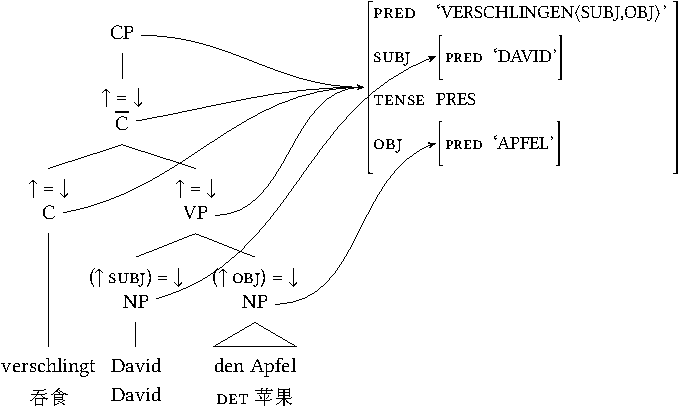
\includegraphics{Figures/verschlingt-david-den-apfel-lfg-lsp-crop}
}
\caption{\label{Abb-Verbstellung-LFG}遵循\citet[\page 41]{Berman2003a}的动词位置分析}
\end{figure}%

%{\interfootnotelinepenalty=10%
\noindent
在了解了第\ref{Kapitel-PSG}章和第\ref{Kapitel-GPSG}章的短语结构规则后,允许动词短语确实看起来很不自然。
然而这对于LFG来说并不是一个问题,因为分析一个给定的句子,我们只需要保证所有必须要的成分(也只有这些成分)都出现。 
完备性
\isc{完整性}\is{completeness}和一致性
\isc{一致性}\is{coherence}的限制保证了这一点。究竟信息来自何方并不重要。
在图\ref{Abb-Verbstellung-LFG}中,动词信息并不来自于动词短语,而是C结点。
C$'$被下面的一个特殊规则所允准:
\ea
\phraserule{C$'$}{
\rulenode{C\\* \up~=~\down}
\rulenode{VP\\*\up~=~\down}}
\z
在LFG规则中,通常来说只对中心词这一个元素进行`\up~=~\down'标记。在(\mex{0})中,有两个这样的元素,这也是为什么二者同时为其父结点的f-结构提供信息的原因。
动词的中心词域被C扩展了。\lfgsubj 和\lfgobj 的信息来自于动词短语,而\pred 信息则来自于C。 
\isc{扩展的中心语范畴}\is{head domain!extended|)}
\isc{动词末位语言}\is{verb"=final language}

\section{局部语序重列}
\label{Abschnitt-LFG-Umstellung}

在前人的工作中已经讨论过两种
\isc{成分序列|(}\is{constituent order|(}处理局部语序重列的方法\footnote{%
  \citet[\page 20--21]{Kaplan95a}讨论了如何在LFG中设计一个基于ID/LP
\isc{ID/LP语法}\is{ID/LP grammar}形式的语法。
  而GPSG类型的组成成分顺序尚未在LFG框架中得以解决。%
}。
\begin{itemize}
\item 像GB\indexgbc 一样在基本结构中移动论元(详见\citealp{Choi99a-u})
\item 直接在短语规则中允准(详见Berman\citeyear[\S~2.1.3.1]{Berman96a-u};\citeyear{Berman2003a})
\end{itemize}

\noindent
如果我们假设语迹在给定结构的语义解释中是发挥作用的,则第一种分析和基于移动的GB分析有着一样的问题。
在\ref{sec-GB-lokale-Umstellung}中,我们已经讨论过这些问题了。

接下来,我讨论\citet[\S~2.1.3]{Berman96a-u}提出的分析,在某种意义上来说我简化了表示。
动词论元的格和语法功能由词库所决定\citep[\page 22]{Berman96a-u}。
(\mex{1})展示了德语动词verschlingen(吞食)的词汇项信息:\footnote{%
  德语的四个格可以用两个二元特征——{\small GOV}和{\small OBL}——进行表示\citep[\page 22]{Berman96a-u}。
  主格的{\small GOV}为$-$,而{\small OBL}为$-$;宾格的{\small GOV}为$+$,而{\small OBL}为$-$。
  这种类型的表示法使得我们可以仅仅通过部分信息来描述一个格。
  如果我们没有声明{\small GOV}的值,则一个{\small OBL}为$-$的格描述既和主格也和宾格兼容。
  因为下面的讨论并没有使用到这种局部声明的好处,我接下来并没有使用特征分解而是直接使用格信息。
}$^,$\footnote{%
  作为一种替代性分析,也可以从格中推导出一个名词短语的语法功能(\citealp[\page 37]{Berman2003a}的德语分析;\citealp[\page 187, \page 201]{Bresnan2001a}的德语和俄语分析\il{Russian})

\ea
\label{Kasus-Implikation-Berman}
\upshape      (\downsp \case) = \mdacc{} $\Rightarrow$ (\upsp \lfgobj) = \down{}
\z

\noindent
  \citet[\S~2.1]{Karttunen89a-u}在分析芬兰语的时候,基于范畴语法\indexcxgc 的框架提出了类似的分析。
  因为格并不总是非常可靠地与语法功能耦合在一起,因此类似的分析并非完全没有问题。
  在德语中,和时间宾格(ii.a)一样,有一些动词会有两个宾格宾语(ii.b--c)和谓词性宾格(ii.d)。

\eal
\ex 
\gll Er arbeitete den ganzen Tag.\\
%	 he worked the.\acc{} whole.\acc{} day\\
     他 工作 DET.\acc{} 整个.\acc{} 一天\\
\ex 
\gll Er lehrte ihn den Ententanz.\\
% he taught him.\acc{} the.\acc{} duck.dance\\
     他 想 他.\acc{} DET.\acc{} 鸭子.跳舞\\
\ex 
\gll Das kostet ihn einen Taler.\\
%	 that costs him.\acc{} a.\acc{} taler\\
     那 花费 他.\acc{} 一.\acc{} 泰勒\\
\ex 
\gll Sie nannte ihn einen Lügner.\\
%	 she called him.\acc{} a.\acc{} liar\\
     她 称 他.\acc{} 一.\acc{} 说谎者\\
\zl
所有的这些宾格都可以出现在长距离依存关系中(见\ref{Abschnitt-NLA-LFG}):

\ea
\gll Wen glaubst du, dass ich getroffen habe.\\
%    who believe you that I met have\\
    谁 相信 你 CONJ  我 会见 AUX \\
\glt `你认为我和谁见面了?'
\z

\noindent
wen(谁)并不是glauben(会见)的宾语,因此并不在glauben的f-结构中。
必须对(i)中的蕴涵规则的右面部分进行修改,允许多种语法功能的析取,还需要解释宾格可以来自于一个嵌入得很深的f-结构这一语言事实。
%}
\ea
\label{le-verschlingen}
\catlexentry{verschlingt}{V}{(\up\ \pred) = {\small `VERSCHLINGEN\arglist{\lfgsubj, \lfgobj}'}\\*
                             (\up\ \lfgsubj{} {\small AGR CAS}) = NOM\\*
                             (\up\ \lfgobj{} {\small AGR CAS}) = ACC\\*
                             (\up\ \lfgtense) = \small PRES}
\z

%\addlines
\largerpage
\noindent
Berman提出一种分析,在这一分析中,动词并不会和它的论元及附接语同时结合,就像GPSG\indexgpsgc 里分析的那样。
她的分析走向另一个极端,她假设动词并不是和附接语或者论元结合,而是直接形成动词短语。
相关的规则如(\mex{1})所示:
\ea
\label{LFG-v-vp}
\phraserule{VP}{
\rulenode{(V)\\* \up~=~\down}}
\z
乍一看来,这种分析非常奇怪,显然一个像devour一样的动词,它自身的分布与它和它论元加和之后的分布是并不相同的。
但是,我们应当回想一下保留下来的针对f-结构一致性与完备性的限制,它们仍然起作用,进而这个理论仍然不会做出错误的(针对语言现象的)预测。
}% footnote breaks

因为动词可以出现在初始位置,它在(\mex{0})规则里被标记为可选(见\ref{Abschnitt-Verbstellung-LFG})。

下面的规则可以用以进一步组合动词和它的主语或者宾语。
\ea
\label{lfg-vp-regel}
\phraserule{VP}{
\rulenode{NP\\* (\upsp \lfgsubj|\lfgobj|\objtheta) = \down}
\rulenode{VP\\* \up~=~\down}}
\z
这里的|
\isc{$\vert$}\is{$\vert$}表示析取(disjunction
\isc{析取}\is{disjunction}),也就是说,NP既可以是相应f-结构的主语也可以是宾语。
因为VP既出现在(\mex{0})中所示规则的左边也出现在其右边,它可以多次进行应用。
而这个规则并不完整。例如,我们还必须解释介词型宾语、小句型论元、形容词性论元和附接语。
参见第\pageref{fn-zp}页的脚注\ref{fn-zp}。

\largerpage
图\vref{Abb-SOV-LFG}展示了(\mex{1}a)的分析。 
\eal
\ex 
\gll {}[dass] David den Apfel verschlingt\\
%      \spacebr{}that David the apple devours\\
      CONJ David DET 苹果 吞食\\
%\glt `that David is devouring the apple'
\glt `David正在吞食苹果'
\ex 
\gll {}[dass] den Apfel David verschlingt\\
     %\spacebr{}that the apple David devours\\
     CONJ DET 苹果 David 吞食 \\
\zl
\begin{figure}
\centerline{%
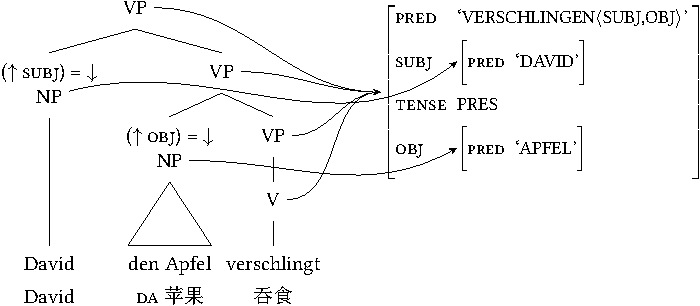
\includegraphics{Figures/david-den-apfel-verschlingt-lfg-lsp-crop}
}
\caption{\label{Abb-SOV-LFG}参考\citet{Berman96a-u}的针对SOV语序的分析}
\end{figure}%
(\mex{0}b)的分析见图\vref{Abb-OSV-LFG}。
\begin{figure}
\centerline{%
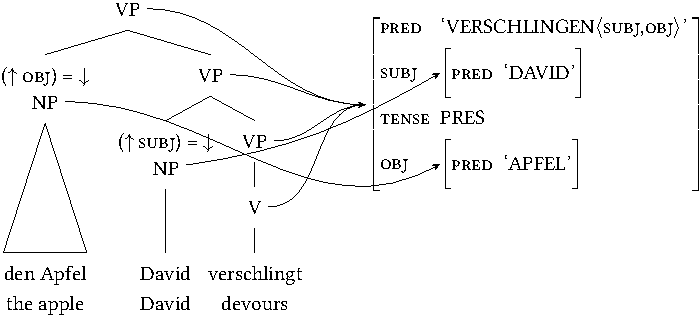
\includegraphics{Figures/den-apfel-david-verschlingt-lfg-lsp-crop}
}
\caption{\label{Abb-OSV-LFG}参考\citet{Berman96a-u}的针对OSV语序的分析}
\end{figure}%
(\mex{0}b)的分析不同于(\mex{0}a)之处仅在于做主语的NP结点与做宾语的NP结点与VP结合的次序不同。\todostefan{fix the arrows, should not cross SUBJ and OBJ}

另外一个必须讨论的情况是:在规则(\ref{LFG-v-vp})中,动词是可选的。
如果它被删去,则VP为空。
这样一来,(\ref{lfg-vp-regel})中的VP规则则允许其右侧有一个空的VP。
这个VP同样可以被删去,尽管规则(\ref{lfg-vp-regel})中并没有做可选的标记。
也就是说,结合语法中其它的可与之交互的规则,相应的符号变成可选的。 
\isc{成分序列|)}\is{constituent order|)}  

\section{长距离依存和功能多变性}
\label{Abschnitt-NLA-LFG}

我们
\isc{长距离依存}\is{long"=distance dependency|(}已经知道了LFG可以解释被动、局部语序重列、不基于转换的动词替换的语言现象。
在讨论GPSG的\ref{Kapitel-GPSG},我们已经看到了如何使用一个不基于转换的分析来处理长距离依存。
在LFG中,\citet{KZ89a}提出了另外一种不基于转换的长距离依存分析,接下来,我们对这种分析展开讨论。

<HERE>
\addlines[-1]
在例(\mex{1})中,不出现的成分Chris(人名)有两个功能:
\ea
\label{ex-Chris-we-think}
\gll Chris, we think that David saw.\\
Chris 我们 认为 CONJ David  看见\\
\glt `Chris,我们认为David看见了。'
\z
首先,假定Chris出现在一个较为普通的句子中,它应该出现在一个不同的位置(前述例子中saw(看见)的\lfgobj 功能),此处,Chris也有这样的功能。
另外,它应该有一个篇章功能(discourse function):
这种构式中的一种特定的信息结构层面的状态(information"=structural status)信息(主句中的话题(\textsc{topic}))。
在LFG中,话题和焦点(\textsc{focus})是语法化的篇章功能(进一步说,\textsc{subj}被视为默认的篇章功能)。
只有语法化的篇章功能才能在f-结构中进行表示,也就是说,那些被特定的句法机制创造出来的并且和句法其它部分相交互的部分。

不像论元功能,篇章功能\textsc{topic}
\isfeat{topic}
\isc{话题}\is{topic}和\textsc{focus}
\isfeat{focus}
\isc{焦点}\is{focus}都不是次范畴的内容,因此并不受完备性和一致性的约束。
像\textsc{topic}和\textsc{focus}篇章功能特征的取值由相应的f-结构的论元功能决定。
(\mex{1})给出了(\ref{ex-Chris-we-think})中的句子的f-结构:

\ea
\lfgms{ pred & `THINK\sliste{ \lfgsubj, comp }' \\
        topic & \rnode{topic}{\lfgms{ pred & `CHRIS' \\
                                   }}\\[4mm]
        subj & \lfgms{ pred & `pro'\\
                     }\\
        comp & \lfgms{ pred & `SEE\sliste{ \lfgsubj, \lfgobj }'\\
                       subj & \lfgms{ pred & `DAVID' \\
                                    }\\
                       obj  & \rnode{obj}{}\\
                     }\\
      }
% todo \nodecurve[r]{topic}[r]{obj}{15em}
\nccurve[ncurv=2.2]{topic}{obj}
\z

\noindent
图中新的连线表示\textsc{topic}的取值和\textsc{comp$|$obj}的取值相等。
在\ref{chap-feature-descriptions}所采用的特征描写中,我用的是带有标号的方块表示特征共享,而不是连线,因为
方块是一种被不同的理论框架广泛采用的标记。
可以用形如(\mex{1})的f-结构限制来形式化如(\mex{0})中的结构共享。 
\ea
\label{Topic-Comp-Obj}
(\upsp  \textsc{topic}) = (\upsp \textsc{comp obj})
\z

\noindent
像(\ref{ex-Chris-we-think})中的前置现象可能发生在不同深度的子句嵌入中。
例(\mex{1}a)是子句嵌入得更浅的一个例子。
宾语和话题出现在同一个f-结构中。
但是(\ref{ex-Chris-we-think})中的宾语来自于think(想)里面的一个从句。

(\mex{1}a)所对应的f-结构如(\mex{1}b)所示:

\eal
\ex 
\gll Chris, we saw.\\
Chirs 我们 看见\\
\glt `Chirs,我们看见了。'
\ex 
\lfgms{ pred & `SEE\sliste{ \lfgsubj, \lfgobj }' \\
        topic & \rnode{topic}{\lfgms{ pred & `CHRIS' \\
                                   }}\\[4mm]
        subj & \lfgms{ pred & `pro'\\
                     }\\
        obj  & \rnode{obj}{}\\
      }
% todo \nodecurve[r]{topic}[r]{obj}{15em}
\nccurve[nodesepA=1pt,ncurv=2.2]{topic}{obj}
\zl

\noindent
这个例子中的\topic{}和\lfgobj 的同一性限制可以按照(\mex{1})来进行形式化:

\ea
\label{Topic-Obj}
(\upsp  \textsc{topic}) = (\upsp \textsc{obj})
\z

\noindent
例(\mex{1}a)是一个比(\ref{ex-Chris-we-think})嵌入程度更深的例子;
(\mex{1}b、c)是相应的f-结构和功能限制。

\eal
\ex 
\gll Chris, we think Anna claims that David saw.\\
Chirs 我们 认为 Anna 声称 CONJ David 看见\\
\glt `Chirs,我们认为Anna声称David看见了。'
\ex 
\lfgms{ pred & `THINK\sliste{ \lfgsubj, comp }' \\
        topic & \rnode{topic}{\lfgms{ pred & `CHRIS' \\
                                   }}\\[4mm]
        subj & \lfgms{ pred & `pro'\\
                     }\\
        comp & \lfgms{ pred & `CLAIM\sliste{ \lfgsubj, comp }\\
                       subj & \lfgms{ pred & `ANNA' \\
                                   }\\
                       comp & \lfgms{ pred & `SEE\sliste{ \lfgsubj, \lfgobj }\\
                                      subj & \lfgms{ pred & `DAVID' \\
                                                   }\\
                                      obj  & \rnode{obj}{}\\
                                    }\\
                     }\\
      }
% todo \nodecurve[r]{topic}[r]{obj}{15em}%
\nccurve[ncurv=2.2]{topic}{obj}
\ex\label{Topic-Comp-Comp-Obj}
(\upsp  \textsc{topic}) = (\upsp \textsc{comp comp obj})
\zl


\noindent
事实上,(\ref{Topic-Comp-Obj})、(\ref{Topic-Obj})以及(\ref{Topic-Comp-Comp-Obj})中的限制是针对c-结构的。
(\mex{1})是把(\ref{Topic-Comp-Obj})结合到c-结构后的示例:
\ea
\begin{tabular}[t]{@{}ccc@{~=~}lc@{}}
CP & $\rightarrow$ & \multicolumn{2}{l}{\hspaceThis{(\upsp \textsc{topic})}XP} & C$'$ \\
 & &  (\upsp \textsc{topic}) & \down & \up~=~\down \\
 & &  (\upsp \textsc{topic}) & (\upsp \textsc{comp obj})\\
\end{tabular}
\z
(\mex{0})声明了第一个组成成分所对应f-结构是其父结点所对应的\textsc{topic}特征的值,此外,这个话题特征的取值也是其补足语小句中的宾语。
我们同样可以找到嵌入深度不同的其他例子。
因此我们需要如(\mex{1})的各种功能限制: 
\eal
\ex (\upsp  \textsc{topic}) = (\upsp \textsc{obj})
\ex (\upsp  \textsc{topic}) = (\upsp \textsc{comp obj})
\ex (\upsp  \textsc{topic}) = (\upsp \textsc{comp comp obj})
\ex \ldots
\zl
可以用(\mex{1})表示这些等式的泛化:
\ea
(\upsp  \textsc{topic}) = (\upsp \textsc{comp* obj})
\z

\noindent
这里,*\isc{*}\is{*}表示\mbox{\small COMP}出现的次数不受限制。
这意味着篇章和语法功能的同一性关系尚待确定,这种性质称为功能多变性(functional uncertainty
\isc{功能的不确定性}\is{functional uncertainty}),见\citew{KZ89a}。

在第\pageref{bsp-fronted-focus}页的针对例(\ref{bsp-fronted-focus})和(\ref{bsp-fronted-topic})的讨论中,
我们知道在英语中并不是只有\textsc{topic}才能放到CP的指定语的位置,\focus 也可以。
我们可以在LFG等式中采用析取符号来表示这种条件:

\ea
(\upsp  \textsc{topic$|$focus}) = (\upsp \textsc{comp* obj})
\z
我们可以引入一个新的特殊符号来替代\textsc{topic$|$focus},表示的是篇章功能的析取:\textsc{df}
\isfeat{df}。
(\mex{0})就此可以简化为(\mex{1}):

\ea
(\upsp  \textsc{df}) = (\upsp \textsc{comp* obj})
\z

\noindent
用于构建英语中前置的c-结构规则最终可以表示如(\mex{1})所示:\footnote{
  注意到\textsc{df}分别对应的这两个析取原则上是独立的。
  而我们并不希望这样。
  我们希望讨论的是父结点所对应的f-结构中的话题“或”焦点,而不是话题“和”焦点。
  所以需要额外的机制来确保\textsc{df}指的是同一个篇章功能。
}
\ea
\begin{tabular}[t]{@{}ccc@{~=~}lc@{}}
CP & $\rightarrow$ & \multicolumn{2}{l}{\hspaceThis{(\upsp \textsc{df})}XP} & C$'$ \\
 & &  (\upsp \textsc{df}) & \down & \up~=~\down \\
 & &  (\upsp \textsc{df}) & (\upsp \textsc{comp* obj})\\
\end{tabular}
\z
在德语中,和宾语一样,几乎任意一个成分(如主语,句子型补足语,附接语)都可以前置。 
而相应的c"=结构规则如(\mex{1})所示:\footnote{\label{fn-zp}%
  在(\mex{1})中,\citet{Berman96a-u}使用的是ZP而不是XP(\mex{1})。
  她形式化了ZP的各种短语结构规则,在这些规则中可以将ZP替换为NP、PP、AP以及各种各样的附接语。
  按照Berman的分析,ZP可以和中间动词结合。
  为了阐述方便,在\ref{Abschnitt-LFG-Umstellung}中,
  我对在VP规则(\ref{lfg-vp-regel})中使用ZP符号持保留态度,选择直接使用NP。
}
\ea
\begin{tabular}[t]{@{}ccc@{~=~}lc@{}}
CP & $\rightarrow$ & \multicolumn{2}{l}{\hspaceThis{(\upsp \textsc{df})}XP} & C$'$ \\
 & &  (\upsp \textsc{df}) & \down & \up~=~\down \\
 & &  (\upsp \textsc{df}) & (\upsp \textsc{comp* gf})\\
\end{tabular}
\z
这里,\textsc{gf}是语法功能的析取,可以出现在前域中。 
\isc{长距离依存}\is{long"=distance dependency|)}

\section{总结与分类}

LFG是一种基于限制的理论,采用了特征描写和短语结构规则。
语法功能被视为理论的原子概念,这一点也将LFG与本书中所介绍的其他理论区别开来。
语法功能并不是像GB那样通过结构关系来进行定义的。
LFG是一种词汇主义理论。像GPSG一样,LFG不需要转换。
影响到论元结构的过程,如被动等,是通过词汇规则进行分析的。
GPSG处理长距离依存是通过所谓的信息在句法树上向上传递进行的,而LFG使用功能多变性:f-结构中的一个部分可以和其内嵌不定深度的另一个f-结构同一。
一致性
\isc{一致性}\is{coherence}和完备性
\isc{完整性}\is{completeness}保证了长距离依存可以被正确消解,也就是说,它保证了一个前置的宾语并不会分配给
一个已经有了宾语或者并不允准宾语的f-结构。

尽管LFG包含一个短语结构模块,和其他语法模型相比,这个模块的作用要小一些。
有一些规则里所有的成分都是可选的。
为了处理一些语言,研究人员甚至提出了一些连成分范畴都不确定的规则(参见\ref{sec-Diskussion-X-Bar})。
在这些语法中,f-结构、一致性、完备性共同保证了语法只能允准良形式的结构。

LFG和诸如\hpsgc、\cxgc 的一些变体等理论不同之处在于特征结构并没有做类型化。
因此,无法通过类型层级表示泛化。
直到最近几年,基于继承关系(inheritance hierarchies
\isc{承继}\is{inheritance})的知识层级化组织都不是理论分析的一部分。
在计算机实现中,虽然可以借助宏(macros
\isc{宏语}\is{macro}),但这只是为一组限制提供一个简称的方式,没有任何理论模块与之相对应。
也可以将宏组织成一个层级结构,\citew*{DKK2004a}讨论了基于这种方式如何捕捉语言知识的泛化性质。
\citet*{ADT2008a}则认为宏不仅可以用来组织词汇项,还可以捕捉c-结构上的增广标注的泛化性。
因为这些发展,LFG和诸如HPSG和CxG的其他理论有趋同发展的趋势。

\citet{Williams84a}比较了GB和LFG中的分析。
他的研究表明很多分析本身是可以互相转化的:LFG中的f-结构的功能可以通过GB中的题元准则(Theta"=Criterion
\isc{$\theta$-理论@$\theta$-理论}\is{theta-theory@$\theta$-Theory}
\isc{$\theta$-准则@$\theta$-准则}\is{theta-criterion@Theta"=Criterion})和格理论(
\isc{格}\is{case}
\isc{格语法}\is{Case Theory})进行分析处理。
LFG可以显性地区分主语和非主语。
在GB中则是区分外部
\isc{外部论元}\is{argument!external}和内部
\isc{内部论元}\is{argument!internal}论元(参见\citealp[\S~1.2]{Williams84a})。
对于GB的一些变体来说,和HPSG\indexhpsgc 以及CxG\indexcxgc 类似,带有主语性质的论元(如果有的话)要做显性标记\citep{Haider86,HM94a,Mueller2003e,MR2001a}。
这个特殊的论元被称之外指定的论元(designated argument\isc{指派论元}\is{argument!designated})。
在不定式中,主语经常在不定式短语的内部缺失。
尽管如此,没有表达出来的主语经常是和主句里的一个论元共指。

\eal
\ex 
\gll Er versucht, [das Buch zu lesen].\\
	 他 尝试 \spacebr{}DET 书 INF 读\\
\glt `他试着读这本书。'
%	 he tries \spacebr{}the book to read\\
%\glt `He is trying to read the book.'
\ex 
\gll Er zwingt ihn, [das Buch zu lesen].\\
	 他 逼迫 他 \spacebr{}the 书 INF 读\\
\glt `他逼着他读这本书。´
%	 he forces him \spacebr{}the book to read\\
%\glt `He is forcing him to read the book.´
\zl 
这是一个所有理论都需要去捕捉的语言事实,也就是说每一种理论都必须区分主语和非主语。

参阅\citew{Kuhn2007a}以了解更多的GB/Minimalism与LFG/HPSG的异同。

\section*{思考题}

\begin{enumerate}
\item 术语“一致性”和“完备性”的具体含义是什么?
\item 什么是扩展的中心词域?
\item 词汇完整性(lexical integrity)的含义是什么? 
\end{enumerate}

\section*{练习题}

\begin{enumerate}
\item 给出kannte(“知道”的过去式)的词汇项描写.
\item 如何分析下面的句子?
\ea
\gll Den Apfel verschlingt David.\\
	 DET 苹果 吞食 David\\
\glt `David在吞食苹果。'
%	 the apple devours David\\
%\glt `David devours the apple.'
\z
提供必要的c-结构规则。
什么样的f-结构被允准?
画出句法树及其对应的f-结构。
对于前置的成分,仅需要画出NP而不需要扩展XP结点。
针对NP的c-结构规则同样可以省略,这样的省略可以在树上通过三角形进行表示。
\end{enumerate}

\section*{延伸阅读}

\ref{Abschnitt-Format-LFG}的讨论主要基于\citet{Dalrymple2001a-u,Dalrymple2006a}。
此外,我还从Jonas Kuhn2007年起使用的教学资料中选取了内容。
\citew{Bresnan2001a}针对英语进行了全面讨论,适合有基础的读者。
\citew{Berman96a-u,Berman2003a}针对德语做了更深入的LFG分析。
\citew{SdA2016a-u}则使用法语例子对LFG进行了介绍。
作者们展示了如何使用XLE系统来开发一部法语\il{French}LFG语法。
这本参考书也讨论了如何使用XLE系统中的有限状态词法分析模块。

\citet{Levelt89a}基于LFG提出了一个语言加工模型。
\citet{Pinker84a-u}——语言习得领域最为知名的学者之一——使用LFG作为他习得理论的模型。
\citew{Pienemann2005a}则针对第一语言与第二语言习得提出了另外一种LFG模型。 


%      <!-- Local IspellDict: en_US-w_accents -->
